\documentclass[10pt]{article}
\usepackage{icmlko}

\icmlmeta{IP 파운데이션 월드모델}{130}{달력이 수요를 이겼다}{팝업 일평균을 정하는 것을 갈라 봤더니 수요도 장소도 아니었다 --- 그리고 그 답이 새 축 한 벌을 낳았다}

\begin{document}

\twocolumn[
\icmlheader

\begin{abstract}
노트 129에서 팝업만 검색 축의 덕을 못 본다는 것을 확인하고 원인을 갈랐다.
팝업의 일평균 방문자를 무엇이 정하는지 \emph{수요 · 공급 · 달력}으로 나눠
재 봤다. \textbf{달력이 이겼다} --- 주말 비중 $+$0.427, 500m 내 경쟁
$+$0.313, 공휴일수 $+$0.251, 장소 유동 $+$0.219, 그리고 오픈 전 검색이
$+$0.088로 꼴찌다. 브랜드가 얼마나 알려졌느냐보다 \textbf{언제 여느냐}가
다섯 배 세다. 그래서 달력을 축으로 만들었다 --- 요일(주기 좌표 둘) · 주말 ·
계절(둘) · 장기연휴까지의 거리. \textbf{수집 비용이 0이고 전 도메인 100\%
덮인다.} 검색 축이 로마자 제목 때문에 0\%였던 만화 · 세계애니까지 덮는다.
\textbf{그런데 모형 계열이 갈렸다.} 부스팅은 오르고(판 $\rho$ $+$0.4107
$\to$ \textbf{$+$0.4203}, 귀무 0.0630 $\to$ \textbf{0.0579}, $z$ $+$6.57
$\to$ \textbf{$+$7.31}) 짝 순위 우도는 내린다($+$0.3891 $\to$ $+$0.3565).
달력 하나만 붙이면 선형은 $+$0.3464에서 $+$0.3092까지 떨어진다. \textbf{같은
축이 모형마다 다른 값을 한다.} 이유를 ``부호가 도메인마다 갈려서''로 잡고
검정했는데 \textbf{틀렸다} --- 부호 일치 80\% 이상만 골라 쓰면 오히려 조금
낮다($+$0.3527 대 $+$0.3565). 세 노트째 내 가설이 무너졌고, 남는 것은
관측뿐이다. 곁가지로 하나 접었다. 만화 · 세계애니에 한국어 제목을 붙이려고
다국어 임베딩 매칭을 만들었는데, 정확도 90\%를 얻으려면 덮음이 6\%로
떨어져 값이 안 나온다.
\end{abstract}
]

\begin{figure}[t]
\centering
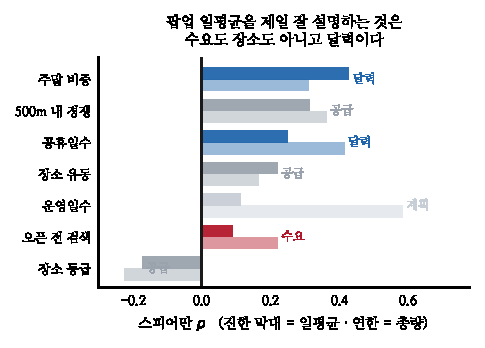
\includegraphics[width=\columnwidth]{figs/supply.pdf}
\caption{진한 막대가 일평균, 연한 막대가 총량. 일평균 쪽에서는 달력이 제일
세고 오픈 전 검색이 제일 약하다.}
\end{figure}

\section{팝업을 갈라 본다}

노트 128과 129에서 검색 축이 아홉 도메인 중 팝업에서만 손해였다. 노트
129에서 ``라벨이 일평균이라 그렇다''는 설명을 세웠다가 스스로 무너뜨렸다
--- 총량으로 바꿔도 음수였다. 그래서 설명을 찾지 말고 \emph{무엇이 실제로
일평균을 정하는지} 갈라 재기로 했다.

세 갈래로 나눴다. \textbf{수요}(오픈 전 검색), \textbf{공급}(장소 유동 ·
장소 등급 · 평수 · 주변 경쟁), \textbf{달력}(주말 비중 · 공휴일수).

\begin{table}[t]
\centering\tsize
\caption{팝업 방문자와의 스피어만. 전부 오픈 이전에 알 수 있는 값이다.}
\begin{tabular}{lrrl}
\toprule
& 일평균 & 총량 & \\
\midrule
주말 비중 & \textbf{$+$.427} & $+$.311 & 달력 \\
500m 내 경쟁 & $+$.313 & $+$.362 & 공급 \\
공휴일수 & $+$.251 & $+$.414 & 달력 \\
장소 유동 & $+$.219 & $+$.165 & 공급 \\
운영일수 & $+$.114 & \textbf{$+$.583} & 계획 \\
오픈 전 검색 & $+$.088 & $+$.220 & 수요 \\
장소 등급 & $-$.173 & $-$.225 & 공급 \\
\bottomrule
\end{tabular}
\end{table}

\claimx{\textbf{언제 여느냐가 누구인가보다 다섯 배 세다.} 일평균 방문자와의
상관이 주말 비중 $+$0.427 대 오픈 전 검색 $+$0.088이다. 브랜드 인지도가
팝업 유입을 못 예측한다는 노트 129의 관측은 ``검색이 나쁘다''가 아니라
``이 라벨이 애초에 달력이 지배하는 양''이라는 뜻이었다.}{$n$은 61$\sim$75로
작다. 표준오차가 0.12쯤이니 $+$0.427과 $+$0.313 사이는 안 갈린다. 갈리는
것은 맨 위와 맨 아래다.}

한 가지가 눈에 걸린다. \textbf{주변 경쟁이 양수다}($+$0.313). 500m 안에
동시 운영 중인 팝업이 많을수록 방문자가 많다 --- 잠식이 아니라 \emph{동네가
붐빈다}는 뜻으로 읽힌다. 경쟁 변수가 실은 입지 품질의 대리였다.

\section{달력을 축으로 만든다}

달력이 팝업에서 제일 세다면, 그리고 노트 126이 ``전 도메인 공통 축만
값어치가 있다''고 했다면, 물어볼 것은 하나다. \emph{달력은 공통인가?}

공통이다. 어느 작품이든 언제 나오는지는 있다.

\begin{table}[t]
\centering\tsize
\caption{달력 축 여섯. 전부 오픈 훨씬 전에 확정된다.}
\begin{tabular}{ll}
\toprule
요일 & 내는 날의 요일 (주기 좌표 둘) \\
주말 & 금 · 토 · 일에 시작하나 \\
계절 & 달 (주기 좌표 둘) \\
연휴 & 가장 가까운 장기연휴 블록까지 거리 \\
\bottomrule
\end{tabular}
\end{table}

\claimx{\textbf{수집 비용 0, 전 도메인 100\% 덮음.} 검색 축은 API 724회를
쓰고도 덮음이 31$\sim$89\%였고 만화 · 세계애니는 로마자 제목 때문에 0\%였다.
달력은 이미 들고 있는 날짜에서 계산된다.}{그래서 ``새 정보''인지는 따로
봐야 한다 --- 공짜라는 것이 값어치를 뜻하지는 않는다.}

도메인 안에서 재면 제일 센 것이 \emph{장기연휴까지의 거리}다 --- 게임
$+$0.373, 애니 $+$0.278, 펀딩 $+$0.264, 도서 $+$0.247, 웹툰 $+$0.212.
아이돌만 $-$0.403으로 반대다(발매 요일이 관행으로 굳어 있다).

\begin{figure*}[t]
\centering

\includegraphics[width=\textwidth]{figs/ladder.pdf}
\caption{축을 더해 온 사다리. 부스팅(F8)은 계속 오르는데 짝 순위
우도(F9)는 달력에서 꺾인다. 귀무 폭은 둘 다 계속 좁아진다.}
\end{figure*}

\section{같은 축이 모형마다 다른 값을 한다}

\begin{table}[t]
\centering\tsize
\caption{판 $\rho$ · 배포 규약 $T$=2025.0 · 가드 일곱 통과.
괄호는 치환 귀무 폭.}
\begin{tabular}{lrr}
\toprule
축 세트 & F8 부스팅 & F9 짝 순위 \\
\midrule
공통 다섯 & $+$.3363 (.079) & $+$.3464 (.135) \\
$+$달력만 & $+$.3376 (.061) & $+$.3092 (.107) \\
$+$검색 & $+$.4107 (.063) & \textbf{$+$.3891} (.104) \\
$+$검색 $+$달력 & \textbf{$+$.4203} (.058) & $+$.3565 (.090) \\
\bottomrule
\end{tabular}
\end{table}

\claimx{\textbf{달력은 트리에서만 값을 한다.} 부스팅은 검색 위에 달력을
얹으면 $+$0.4107에서 $+$0.4203으로 오르는데, 짝 순위 우도는 $+$0.3891에서
$+$0.3565로 내린다. 달력만 붙이면 선형은 $+$0.3464에서 $+$0.3092까지
떨어진다.}{모형 둘의 사례다. 다른 선형 모형(F6 직접 풀링)도 같은 방향으로
움직였다($+$0.3843 $\to$ $+$0.3513).}

이유를 짐작했다. 달력 효과는 주기적이고 도메인마다 방향이 다르니(아이돌만
연휴 거리가 음수다) 공유 계수 하나로는 못 담고, 트리는 도메인 표시자로
쪼갤 수 있다. 그럴듯해서 검정했다.

\claimx{\textbf{틀렸다.} 축마다 도메인 사이 부호 일치율을 재고 80\% 이상만
골라 썼더니 오히려 조금 낮다 --- 짝 순위 우도가 전부 쓸 때 $+$0.3565,
골라 쓸 때 $+$0.3527이다. 부호 일치가 기제가 아니다.}{일치율은 도메인
넷 이상에서 잰 것이고 도메인 수가 7$\sim$10으로 적다. 더 나은 기제 설명은
아직 없다 --- 관측만 남긴다.}

노트 128 이후 세 노트째 내가 세운 설명이 무너졌다(팝업 규모/강도, 웹툰
결합, 부호 일치). 셋 다 그럴듯했고 셋 다 검정에서 죽었다. 하네스를 방법에서
떼어 놓은 값이 여기서 나온다 --- 설명이 틀려도 수치는 남는다.

\section{사다리}

\begin{table}[t]
\centering\tsize
\caption{부스팅의 궤적. 축을 더할 때마다 셋이 같이 좋아진다.}
\begin{tabular}{lrrr}
\toprule
& 판 $\rho$ & 귀무 폭 & $z$ \\
\midrule
공통 다섯 & $+$.3363 & .0789 & $+$4.41 \\
$+$검색 (웹툰 뺌) & $+$.4019 & .0752 & $+$5.39 \\
$+$검색 (웹툰 넣음) & $+$.4107 & .0630 & $+$6.57 \\
$+$검색 $+$달력 & \textbf{$+$.4203} & \textbf{.0579} & \textbf{$+$7.31} \\
\bottomrule
\end{tabular}
\end{table}

\claimx{\textbf{맞히기가 오르면서 귀무가 같이 좁아진다.} 보통 축을 늘리면
모형이 유연해져 우연히 잘 보일 길도 늘어나는데 여기서는 반대다. 전 도메인이
공유하는 축이라 한 도메인의 표류에 덜 노출된다 --- 노트 126의 법칙이
경계하던 방향의 정확한 반대편이다.}{한 시간 분할 한 판이다. 그리고 이
사다리는 부스팅 하나의 것이다 --- 짝 순위 우도는 마지막 칸에서 꺾인다.}

\section{접은 것 --- 한국어 제목 매칭}

만화 · 세계애니는 제목이 로마자뿐이라 검색 축 덮음이 0\%다. 애니 도메인이
라프텔이라 한국어 제목을 2{,}073건 들고 있으니 옮겨 오려 했다. 다국어
임베딩 $+$ 방영일 창 $+$ 상호 최적 매칭으로 짜고, 예전 세션이 남긴 짝
42개로 검정했다.

\begin{table}[t]
\centering\tsize
\caption{한국어 제목 매칭 --- 정확도를 사려면 덮음을 판다.}
\begin{tabular}{lrr}
\toprule
문턱 & 붙은 것 & 정확도 \\
\midrule
0.55 & 398 & .769 \\
0.75 & 314 & .833 \\
0.85 & \textbf{177} & \textbf{.909} \\
0.90 & 97 & .909 \\
\bottomrule
\end{tabular}
\end{table}

\claimx{\textbf{값이 안 나와서 접었다.} 정확도 90\%를 얻으려면 덮음이
177/2{,}988 $=$ 6\%로 떨어진다. 세계애니 후행 300건 중 열여덟 건쯤에
축이 붙는 셈이다. 게다가 그 90\%조차 열한 쌍 위에서 잰 값이라 구간이
59$\sim$100\%다.}{만화는 대응 저장소가 아예 없어 완전히 막혀 있다. 코드는
남겨 뒀다 --- 라프텔 쪽 자료가 늘면 다시 볼 만하다.}

\section{남은 것}

\begin{table}[t]
\centering\tsize
\caption{다음.}
\begin{tabular}{ll}
\toprule
웹툰 & 덮음 37.9\% $\to$ 나머지 (할당량 회복 후) \\
달력 & 왜 트리에서만 되는지 --- 기제가 아직 없다 \\
팝업 & 일평균 대신 무엇을 예측할지가 제품 질문이다 \\
\bottomrule
\end{tabular}
\end{table}

마지막 줄이 이번 노트에서 제일 큰 것일지도 모른다. 팝업 일평균은 달력이
지배하는 양이고, 기획에서 바꿀 수 있는 것(브랜드 · 굿즈 · 체험)이 아니라
\textbf{언제 여느냐}가 대부분을 설명한다. 그렇다면 제품이 물어야 할 것은
``이 팝업이 하루에 몇 명을 받나''가 아니라 다른 것일 수 있다.

\end{document}
